\documentclass[11pt,a4paper]{article}

\usepackage[utf8]{inputenc}
\usepackage[T1]{fontenc}
\usepackage{amsmath,amssymb}
\usepackage{booktabs}
\usepackage{listings}
\usepackage{graphicx}
\usepackage[margin=2.5cm]{geometry}
\usepackage{hyperref}
\usepackage{xcolor}

\hypersetup{
  colorlinks=true,
  linkcolor=blue!50!black,
  urlcolor=blue!50!black,
  citecolor=blue!50!black
}

\graphicspath{{figures/}{docs/figures/}}

\lstset{
  basicstyle=\ttfamily\small,
  columns=fullflexible,
  keepspaces=true,
  breaklines=true,
  extendedchars=true,
  frame=single,
  literate={θ}{{$\theta$}}1
           {á}{{\'a}}1 {é}{{\'e}}1 {í}{{\'i}}1 {ó}{{\'o}}1 {ú}{{\'u}}1 {ñ}{{\~n}}1
           {Á}{{\'A}}1 {É}{{\'E}}1 {Í}{{\'I}}1 {Ó}{{\'O}}1 {Ú}{{\'U}}1 {Ñ}{{\~N}}1
}

\title{Función de utilidad con servicios ecosistémicos\\
       en MimiGIVE-forests}
\author{MimiGIVE-forests}
\date{\today}

\begin{document}
\maketitle

\begin{abstract}
El costo social del carbono (SCC) de GIVE descuenta daños marginales usando
solo el consumo per cápita. Esta nota documenta la extensión implementada en
\texttt{src/scc.jl}: una función de utilidad CES que combina consumo de mercado
\(C_t\) y servicios ecosistémicos no comercializables \(E_t\), y que usa tanto
el nivel de esos servicios como su daño marginal. Se presentan las fórmulas,
las unidades, el tratamiento del periodo 2022--2100 del emulador forestal, la
implementación computacional y un conjunto de pruebas de regresión.
\end{abstract}

\tableofcontents

\section{Motivación}

La fórmula estándar de GIVE para el SCC es
\begin{equation}
  \mathrm{SCC} =
  \sum_{t=y}^{T} \left(\frac{C_y}{C_t}\right)^{\eta}
  \left(\frac{1}{1+\rho}\right)^{t-y} \mathrm{MD}_{t},
  \label{eq:scc-original}
\end{equation}
donde \(C_t\) es consumo neto per cápita, \(\eta\) la aversión a la
desigualdad, \(\rho\) la tasa de preferencia temporal pura y
\(\mathrm{MD}_t\) el daño marginal total por tonelada emitida. Esta fórmula
trata todos los daños como pérdidas de consumo de mercado.

El emulador forestal (\texttt{ForestEmulator}) produce, para cada región de
impacto y año, el valor de cuatro servicios: recreación (\texttt{rec}),
hábitat (\texttt{hab}), productos forestales no maderables (\texttt{nwfp}) y
agua (\texttt{wat}). Los tres primeros son, en su mayoría, servicios no
comercializables; \texttt{nwfp} es un bien de mercado. La extensión incorpora
los servicios no comercializables en una función de utilidad CES y usa su daño
marginal en la suma del SCC.

\section{La función de utilidad CES}

Para cada año \(t\) se define
\begin{equation}
  U_t = \left[(1-s)\,C_t^{\theta} + s\,E_t^{\theta}\right]^{1/\theta},
  \qquad 0 \le s < 1,\quad \theta \neq 0,
  \label{eq:ces}
\end{equation}
donde
\begin{itemize}
  \item \(C_t\) es consumo neto per cápita, en USD2005 por persona y año.
  \item \(E_t\) son servicios ecosistémicos no comercializables per cápita,
        en USD2005 por persona y año.
  \item \(s\) es la participación del servicio ecosistémico en la utilidad.
  \item \(\theta\) controla la curvatura. La elasticidad de sustitución es
        \(\sigma = 1/(1-\theta)\). Para \(\theta \to 0\) el límite es
        Cobb--Douglas; ese caso no está implementado.
\end{itemize}

Las derivadas marginales, que se usan en la suma del SCC, son
\begin{align}
  \mu^C_t \equiv \frac{\partial U_t}{\partial C_t}
  &= (1-s)\,C_t^{\theta-1}\,U_t^{1-\theta},
  \label{eq:muC}\\
  \mu^E_t \equiv \frac{\partial U_t}{\partial E_t}
  &= s\,E_t^{\theta-1}\,U_t^{1-\theta}.
  \label{eq:muE}
\end{align}
Cuando \(s=0\), \(U_t=C_t\), \(\mu^C_t=1\) y \(\mu^E_t=0\), de modo que
\eqref{eq:ces} se reduce exactamente a la fórmula original
\eqref{eq:scc-original}.

\subsection{Bienestar social y SCC}

El bienestar social intertemporal es
\begin{equation}
  W = \sum_{t=y}^{T}
      \left(\frac{1}{1+\rho}\right)^{t-y}
      \frac{U_t^{1-\eta}}{1-\eta}.
  \label{eq:welfare}
\end{equation}
Un pulso de emisiones cambia \(C_t\) y \(E_t\) en
\(\mathrm{MD}_{C,t}\) y \(\mathrm{MD}_{E,t}\), respectivamente. Diferenciando
\eqref{eq:welfare} y normalizando por el valor marginal del consumo en el año
del pulso, \(y\), se obtiene
\begin{equation}
  \boxed{
  \mathrm{SCC} =
  \frac{
    \displaystyle\sum_{t=y}^{T}
    \left(\frac{U_y}{U_t}\right)^{\eta}
    \left(\frac{1}{1+\rho}\right)^{t-y}
    \left[\mu^C_t\,\mathrm{MD}_{C,t}
        + \mu^E_t\,\mathrm{MD}_{E,t}\right]
  }{
    \mu^C_y
  }}
  \label{eq:scc-ces}
\end{equation}
donde \(\mathrm{MD}_{C,t}\) es el daño marginal al consumo de mercado y
\(\mathrm{MD}_{E,t}\) el daño marginal a los servicios ecosistémicos, ambos
por tonelada de gas y en USD2005. Los daños son positivos cuando reducen
\(C\) o \(E\).

Si \(s=0\), \(\mu^C_t=1\), \(U_t=C_t\) y \(\mu^E_t=0\), y
\eqref{eq:scc-ces} es idéntica a \eqref{eq:scc-original}. Esta propiedad se
verifica en las pruebas de regresión.

\section{La variante CES anidada (\texttt{:derivatives})}

El método \texttt{:derivatives} usa una segunda capa CES:
\begin{equation}
  \tilde U_t =
  \left[
    \left((1-s)C_t^{\theta} + sE_t^{\theta}\right)^{\theta_2/\theta}
    + s_2\,i_{pc}^{\theta_2}
  \right]^{1/\theta_2},
  \qquad s_2 \ge 0,\quad \theta_2 \neq 0,
  \label{eq:nested}
\end{equation}
donde \(i_{pc}\) es una escala de numerario (por defecto \(1.0\)). Sea
\begin{equation}
  c_t = \left((1-s)C_t^{\theta} + sE_t^{\theta}\right)^{1/\theta}
\end{equation}
el compuesto de primer nivel. Las derivadas son
\begin{align}
  \frac{\partial \tilde U_t}{\partial C_t}
  &= (1-s)\left(\frac{c_t}{C_t}\right)^{1-\theta}
     \left(\frac{\tilde U_t}{c_t}\right)^{1-\theta_2},
  \label{eq:dfc}\\
  \frac{\partial \tilde U_t}{\partial E_t}
  &= s\left(\frac{c_t}{E_t}\right)^{1-\theta}
     \left(\frac{\tilde U_t}{c_t}\right)^{1-\theta_2}.
  \label{eq:dfe}
\end{align}
El SCC se calcula con \eqref{eq:scc-ces}, reemplazando \(U_t\) por
\(\tilde U_t\) y \(\mu^C,\mu^E\) por las derivadas \eqref{eq:dfc}--\eqref{eq:dfe}.
Con \(s_2=0\), \(\tilde U_t=c_t\) y las ecuaciones \eqref{eq:dfc}--\eqref{eq:dfe}
coinciden con \eqref{eq:muC}--\eqref{eq:muE}; por tanto, los métodos
\texttt{:moore} y \texttt{:derivatives} deben dar el mismo resultado cuando
\(s_2=0\). Esto también se verifica en las pruebas.

\section{Datos, unidades y periodo del emulador}

\subsection{Nivel de servicios ecosistémicos}

\texttt{ForestEmulator} produce \texttt{country\_value} en
\(10^6\) USD2020 por año, para cada país y servicio. El código usa los
servicios no comercializables \(S_{\mathrm{nm}}=\{\texttt{rec},\texttt{hab},
\texttt{wat}\}\) y excluye \texttt{nwfp}, que es un bien de mercado. El nivel
per cápita es
\begin{equation}
  E_t =
  d \cdot 10^6 \cdot
  \frac{\sum_{c}\sum_{s\in S_{\mathrm{nm}}} V_{c,s,t}}{10^6\,P_t}
  =
  d \cdot \frac{\sum_{c,s\in S_{\mathrm{nm}}} V_{c,s,t}}{P_t},
  \label{eq:E}
\end{equation}
donde \(V_{c,s,t}\) está en \(10^6\) USD2020, \(P_t\) es la población global
en millones y
\begin{equation}
  d = \frac{1}{\texttt{pricelevel\_2005\_to\_2020}}
    = \frac{87.504}{113.648}
    \approx 0.7700
\end{equation}
convierte USD2020 a USD2005. El resultado \(E_t\) queda en USD2005 por persona
y año, consistente con \(C_t\).

\subsection{Daño marginal a los servicios ecosistémicos}

El modelo marginal de Mimi ya divide la diferencia entre la simulación con
pulso y la simulación base por el tamaño del pulso. Por eso, al evaluar
\texttt{mm[:ForestEmulator, :country\_value]} se obtiene el cambio por tonelada
de gas. El daño (positivo si el pulso reduce el valor) es
\begin{equation}
  \mathrm{MD}_{E,t} =
  -\, d \cdot \kappa_g \cdot \frac{10^6}{\Delta_g} \cdot
  \sum_{c,s\in S_{\mathrm{nm}}}
  \left(V^{\mathrm{pulso}}_{c,s,t} - V^{\mathrm{base}}_{c,s,t}\right),
  \label{eq:MDE}
\end{equation}
donde \(\Delta_g\) es el tamaño del pulso en unidades físicas
(\(10^9\) tC para CO\(_2\), \(10^6\) t para CH\(_4\) y N\(_2\)O) y
\(\kappa_g\) convierte masa de gas a la unidad del SCC:
\begin{equation}
  \kappa_{\mathrm{CO_2}} = \frac{12}{44}, \qquad
  \kappa_{\mathrm{CH_4}} = 1, \qquad
  \kappa_{\mathrm{N_2O}} = \frac{28}{44}.
\end{equation}
El factor \(10^6\) convierte de \(10^6\) USD a USD. La división por el pulso
en toneladas la hace internamente Mimi; el pulso es \(1\) GtC para CO\(_2\)
(\(10^9\) tC) y \(1\) Mt para CH\(_4\) y N\(_2\)O (\(10^6\) t).
Para CO\(_2\), multiplicar por \(12/44\) convierte USD/tC en USD/tCO\(_2\).

\subsection{Daño marginal al consumo}

\(\mathrm{MD}_{C,t}\) es el daño marginal total del modelo estándar:
agregador de daños (agricultura, energía y mortalidad) más el daño de aumento
del nivel del mar de MimiCIAM, en USD2005 por tonelada de gas. Es el mismo
vector que usa \eqref{eq:scc-original}; no se le resta \(\mathrm{MD}_{E,t}\)
porque los servicios forestales no están incluidos en el agregador de daños.

\subsection{Horizonte temporal}

Las regresiones del emulador están calibradas para 2022--2100. Para poder
evaluar la utilidad en todo el horizonte del modelo (2020--2300) se usa:
\begin{itemize}
  \item \(E_t = E_{2022}\) para \(t<2022\);
  \item \(E_t = E_{2100}\) para \(t>2100\);
  \item \(\mathrm{MD}_{E,t}=0\) fuera de 2022--2100.
\end{itemize}
Es decir, el nivel per cápita de servicios se mantiene constante en los
extremos y no se atribuyen daños forestales adicionales después de 2100.
Esta es una limitación explícita, no un resultado del emulador.

\section{Implementación}

\subsection{API}

La extensión se activa con los argumentos \texttt{method} y \texttt{params}
de \texttt{compute\_scc}:
\begin{lstlisting}
using MimiGIVE

m = MimiGIVE.get_model(socioeconomics_source = :SSP,
                       SSP_scenario = "SSP245",
                       forest_emulator = :jules)

# SCC estándar (sin servicios ecosistémicos)
scc0 = MimiGIVE.compute_scc(m, year = 2020)

# CES de un nivel
scc1 = MimiGIVE.compute_scc(m, year = 2020, method = :moore,
    params = (forest = true, s = 0.10, θ = 0.55))

# CES anidada
scc2 = MimiGIVE.compute_scc(m, year = 2020, method = :derivatives,
    params = (forest = true, s = 0.10, θ = 0.55,
              s2 = 0.10, θ2 = 0.58, i_pc = 1.0))
\end{lstlisting}

Los métodos \texttt{:moore} y \texttt{:derivatives} requieren un modelo
construido con \texttt{forest\_emulator} cuando \texttt{forest = true}, y solo
están disponibles para \texttt{n = 0} (ejecución determinista). Si
\texttt{forest = false} o \texttt{s = 0}, el canal forestal se apaga y el
resultado coincide con el SCC original.

\subsection{Parámetros por defecto}

\begin{lstlisting}
FOREST_DEFAULT_PARAMS = (
    forest = true,
    s      = 0.10,
    θ      = 0.55,
    s2     = 0.10,
    θ2     = 0.58,
    i_pc   = 1.0,
)
\end{lstlisting}

\texttt{sample\_forest\_params(rng)} devuelve una combinación aleatoria de
\(s\), \(\theta\), \(s_2\) y \(\theta_2\) de las tablas usadas en el análisis
de incertidumbre. Los valores de \(\theta\) incluyen casos negativos; el código
admite \(\theta<0\) siempre que \(C_t>0\) y \(E_t>0\), y falla con un mensaje
claro si no se cumple.

\subsection{Validaciones}

\begin{itemize}
  \item \(0 \le s < 1\). El caso \(s=1\) dejaría el consumo con peso cero y
        el numerario del SCC sería \(\mu^E_y\), que no está implementado.
  \item \(\theta \neq 0\) cuando \(s>0\).
  \item \(s_2 \ge 0\); \(\theta_2 \neq 0\) cuando \(s_2>0\).
  \item \(C_t>0\) y \(E_t>0\) en todos los años incluidos en la suma.
  \item El modelo debe contener \texttt{ForestEmulator} cuando
        \texttt{forest = true}.
\end{itemize}

\section{Resultados de referencia y tendencias}

La Tabla~\ref{tab:scc} usa la configuración por defecto de \texttt{compute\_scc}
(incluye SLR), JULES, 2020 y los parámetros centrales \(s=0.10\),
\(\theta=0.55\), \(s_2=0.10\), \(\theta_2=0.58\). Los valores están en USD2005
por tCO\(_2\).

\begin{table}[h]
\centering
\begin{tabular}{lrrrr}
\toprule
Escenario & Original & \texttt{:moore} & \texttt{:derivatives} & \(\Delta\) \texttt{:moore} \\
\midrule
SSP119 & 10.93 & 11.24 & 11.24 & +2.80\% \\
SSP245 & 22.54 & 22.64 & 22.65 & +0.44\% \\
SSP585 & 14.50 & 14.66 & 14.67 & +1.13\% \\
\bottomrule
\end{tabular}
\caption{SCC 2020 con y sin servicios ecosistémicos. La variante
\texttt{:derivatives} usa \(s_2=0.10\), por lo que queda muy cerca de
\texttt{:moore}.}
\label{tab:scc}
\end{table}

La prueba \texttt{test/test\_compute\_utility\_function.jl} usa
\texttt{include\_slr = false}; por eso allí los niveles son algo menores
(SSP245: 22.26 original y 22.36 con \(s=0.10\)). El cambio porcentual es
prácticamente el mismo. La Figura~\ref{fig:paths} muestra las tendencias de la
fórmula CES y de sus insumos.

\begin{figure}[htbp]
\centering
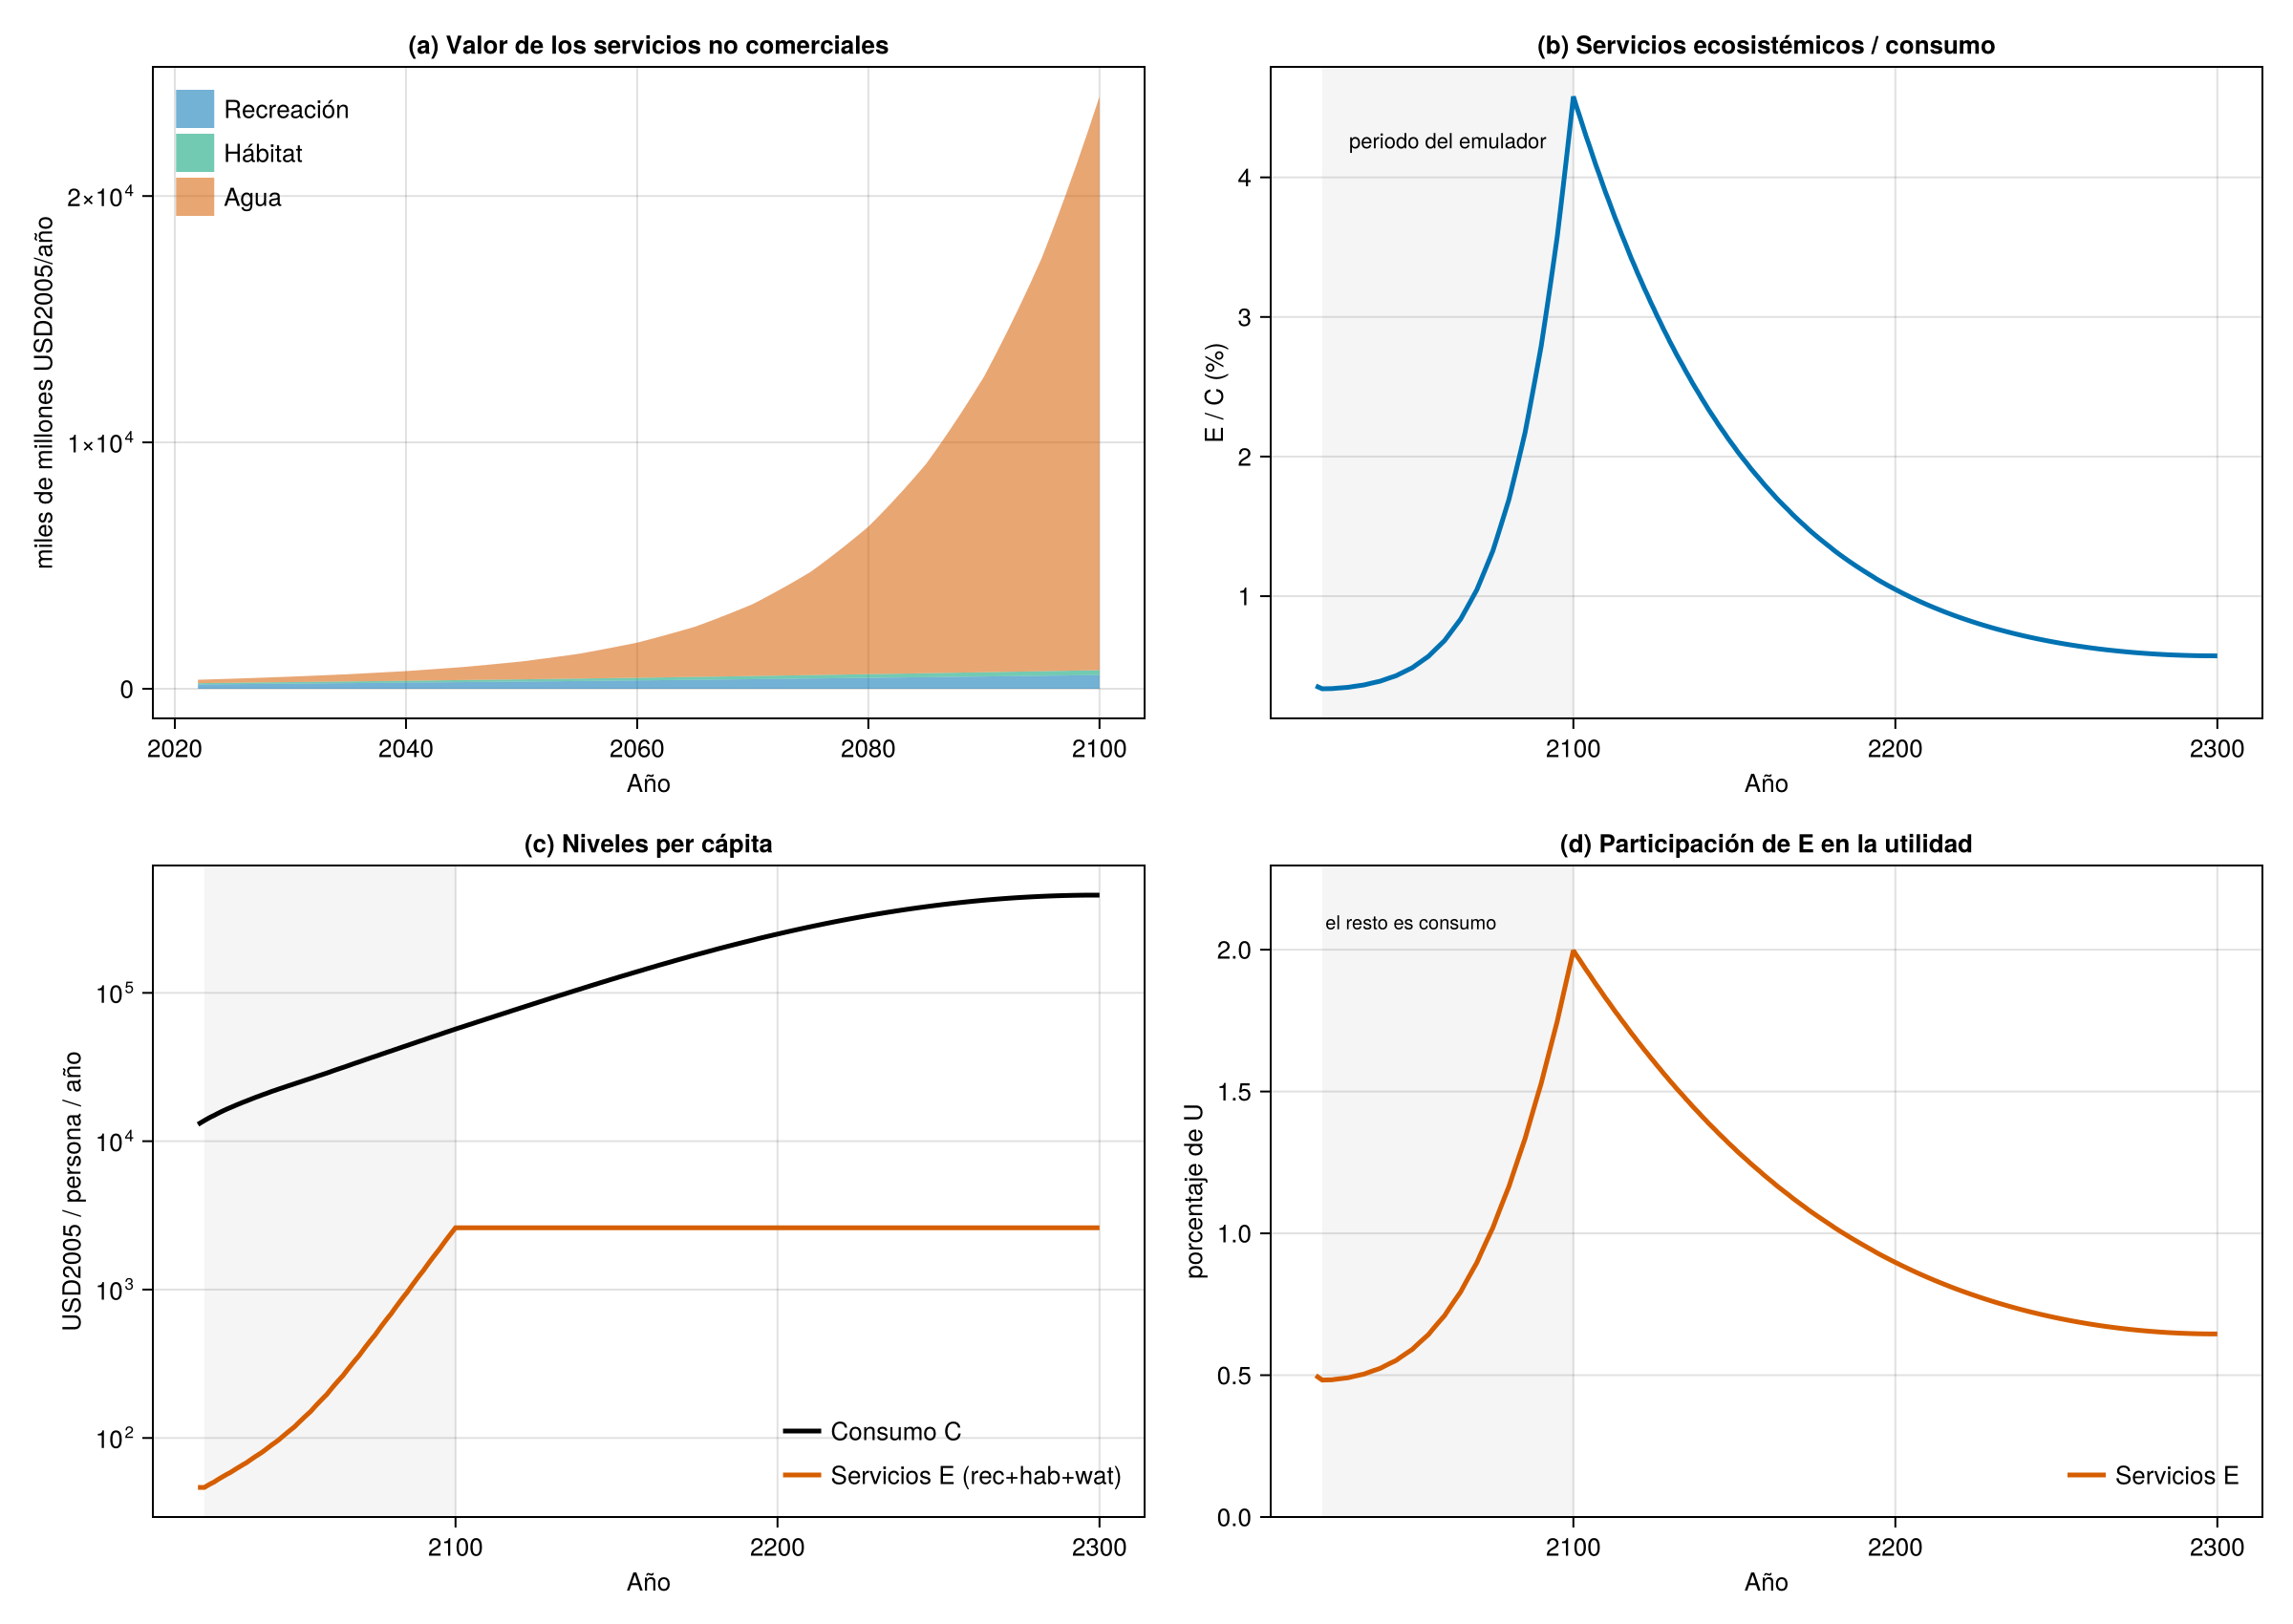
\includegraphics[width=\textwidth]{utility_paths.png}
\caption{Tendencias de la fórmula CES para SSP245, JULES, \(s=0.10\) y
\(\theta=0.55\). (a) Valor global de los servicios no comercializables por
servicio; (b) cociente \(E_t/C_t\); (c) niveles per cápita de \(C_t\) y
\(E_t\) en escala logarítmica; (d) participación de \(E_t\) en la utilidad
\(U_t\). La banda gris marca el periodo 2022--2100 del emulador.}
\label{fig:paths}
\end{figure}

El valor global de los servicios no comercializables es aproximadamente
0.34\% del consumo per cápita en 2022 y alcanza un máximo cercano a 4.6\% en
2100. El servicio de agua domina el valor de 2100 porque su elasticidad ingreso
calibrada es alta (\(2.02\)); los resultados son sensibles a ese supuesto y a
la forma funcional de la valorización. Después de 2100, el nivel per cápita de
\(E\) se mantiene constante y \(\mathrm{MD}_E=0\), de modo que el cociente
\(E/C\) baja a medida que crece el consumo.

\begin{figure}[htbp]
\centering
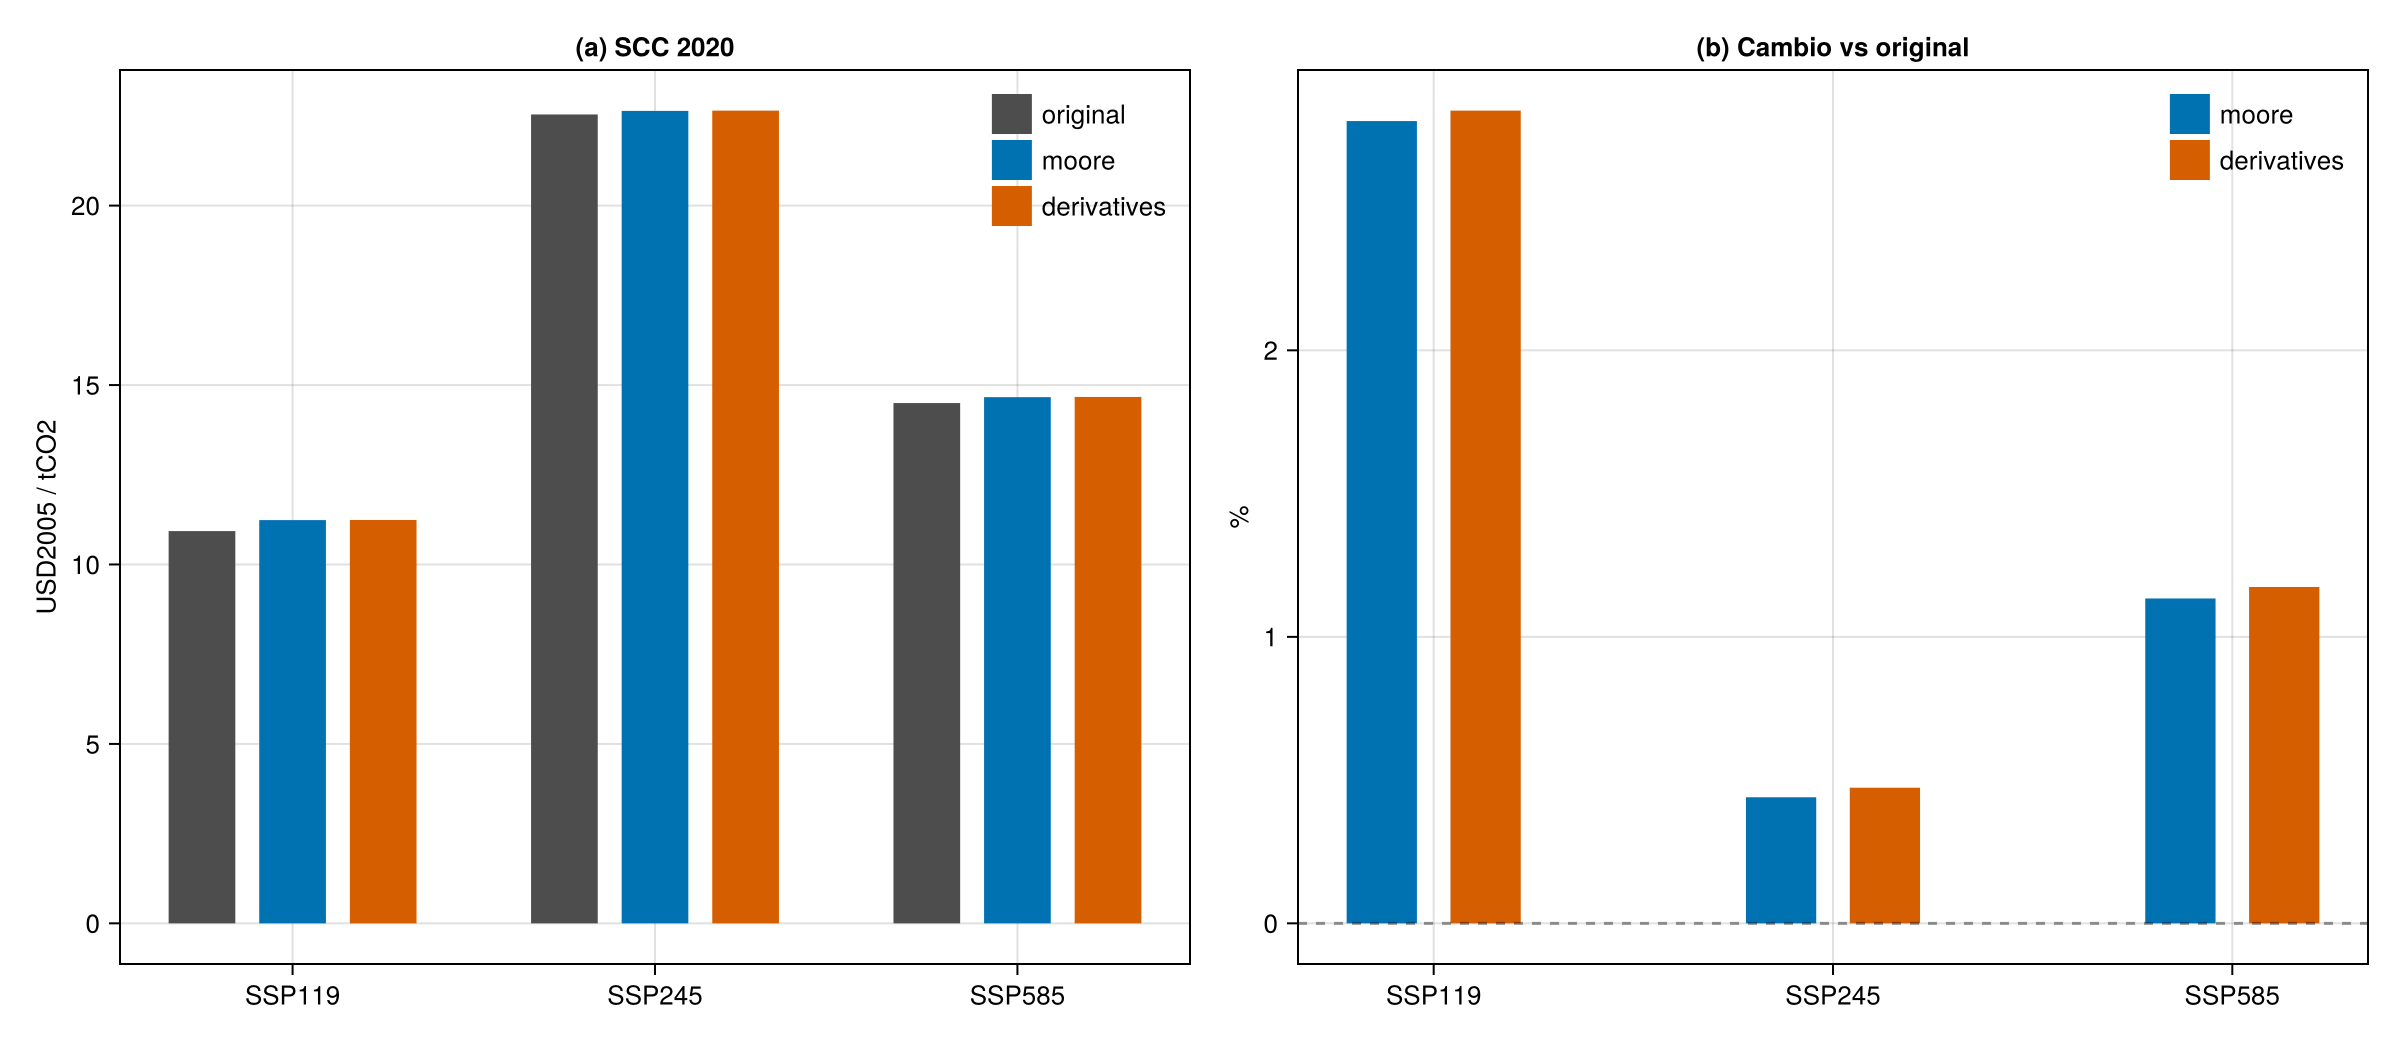
\includegraphics[width=\textwidth]{scc_scenarios.png}
\caption{(a) SCC 2020 por escenario y método; (b) cambio porcentual respecto al
SCC original. JULES, parámetros centrales.}
\label{fig:scenarios}
\end{figure}

El aumento del SCC no es uniforme: es +2.80\% en SSP119, +0.44\% en SSP245 y
+1.13\% en SSP585. La magnitud depende sobre todo de \(\theta\). La
Figura~\ref{fig:sensitivity} y la Tabla~\ref{tab:sensitivity} muestran que, con
mayor sustituibilidad (\(\theta<0\)), el cambio puede ser mucho mayor: hasta
+30.6\% con \(s=0.15\) y \(\theta=-0.16\).

\begin{figure}[htbp]
\centering
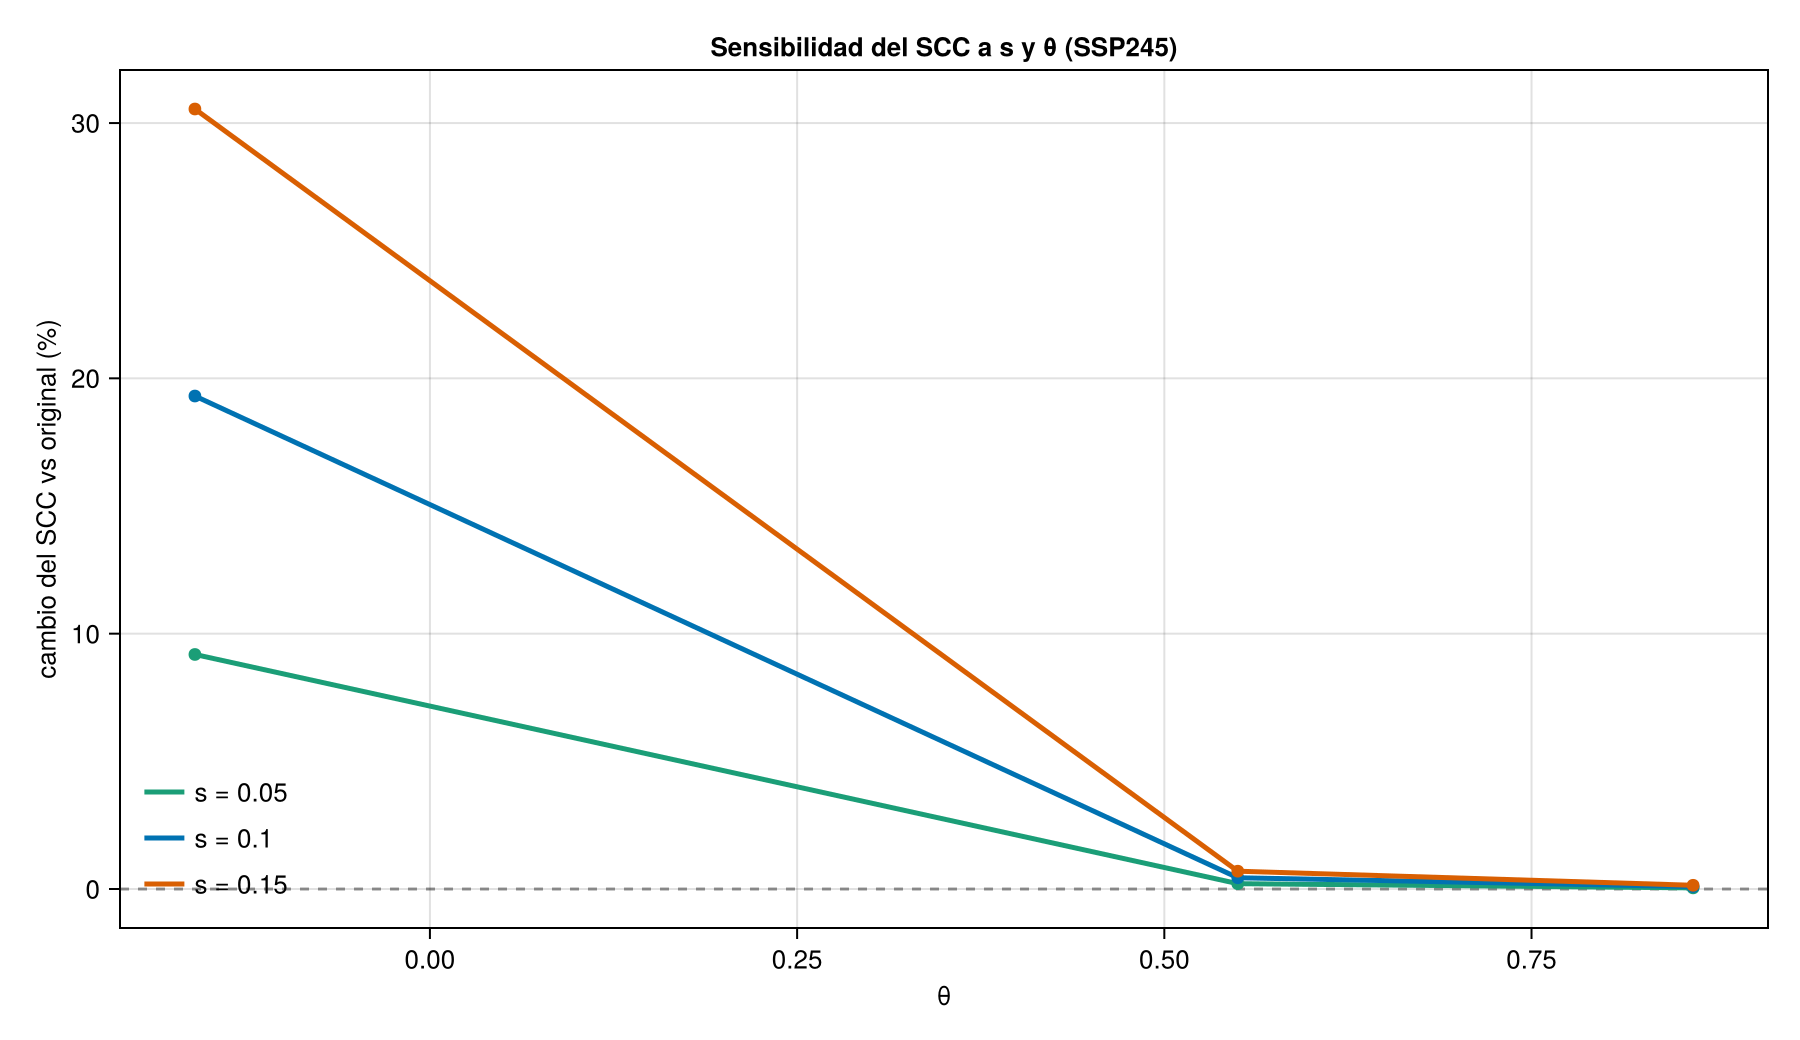
\includegraphics[width=0.8\textwidth]{scc_sensitivity.png}
\caption{Cambio porcentual del SCC \texttt{:moore} respecto al original en
SSP245, para distintos valores de \(s\) y \(\theta\).}
\label{fig:sensitivity}
\end{figure}

\begin{table}[h]
\centering
\begin{tabular}{lrrr}
\toprule
\(s\) & \(\theta=-0.16\) & \(\theta=0.55\) & \(\theta=0.86\) \\
\midrule
0.05 & +9.19\% & +0.21\% & +0.04\% \\
0.10 & +19.31\% & +0.44\% & +0.09\% \\
0.15 & +30.55\% & +0.70\% & +0.15\% \\
\bottomrule
\end{tabular}
\caption{Cambio porcentual del SCC \texttt{:moore} respecto al original,
SSP245, 2020.}
\label{tab:sensitivity}
\end{table}

\subsection{Reproducción}

El script \texttt{scripts/utility\_scc.jl} reproduce la tabla, la sensibilidad
y las tres figuras:
\begin{lstlisting}
julia --project=. scripts/utility_scc.jl
# solo regenerar figuras con los CSV ya calculados:
UTILITY_SCC_REUSE=true julia --project=. scripts/utility_scc.jl
\end{lstlisting}
Los resultados numéricos se guardan en
\texttt{docs/utility\_scc\_results.csv} y
\texttt{docs/utility\_scc\_sensitivity.csv}; las figuras en
\texttt{docs/figures/}. La prueba formal de regresión está en
\texttt{test/test\_compute\_utility\_function.jl} y se ejecuta con la suite de
pruebas del paquete (\texttt{Pkg.test()}).

\section{Supuestos y limitaciones}

\begin{enumerate}
  \item \textbf{Consumidor global representativo.} \(C_t\) y \(E_t\) son
        globales y per cápita. No hay ponderación por equidad entre países en
        esta extensión; los métodos equivalentes con \texttt{discount\_rates}
        y ponderación por equidad no están implementados.
  \item \textbf{Servicios no comercializables.} Solo \texttt{rec},
        \texttt{hab} y \texttt{wat} entran en \(E_t\). \texttt{nwfp} es un
        bien de mercado y no se suma al consumo en esta implementación, por lo
        que su daño no está incluido en el SCC.
  \item \textbf{Fuera de 2022--2100.} El nivel de \(E\) se mantiene constante
        y \(\mathrm{MD}_E=0\). No se extrapola la respuesta climática del
        emulador más allá de su periodo de calibración.
  \item \textbf{Carbono forestal.} El flujo de CO\(_2\) del emulador
        (\texttt{global\_co2\_flow}) no se retroalimenta al ciclo del carbono
        de FAIR; el SCC no incluye ese efecto.
  \item \textbf{Parámetros normativos.} \(s\), \(\theta\), \(s_2\), \(\theta_2\)
        y \(i_{pc}\) no se estiman dentro del modelo. Los valores centrales y
        las distribuciones de \texttt{sample\_forest\_params} son supuestos
        de análisis, no estimaciones únicas.
  \item \textbf{Incertidumbre.} \texttt{compute\_scc} con estos métodos corre
        una sola realización. La incertidumbre de los parámetros de utilidad
        debe explorarse con un bucle externo que llame a
        \texttt{sample\_forest\_params} y \texttt{compute\_scc}; la
        incertidumbre del emulador (coeficientes y elasticidades) se explora
        con el Monte Carlo de \texttt{run\_mcs}.
  \item \textbf{Precio del agua.} La elasticidad ingreso del agua produce un
        crecimiento fuerte de su valor hacia 2100. Cualquier límite o
        corrección de precio es una decisión de modelización separada y no se
        aplica aquí.
\end{enumerate}

\section{Pruebas}

El archivo \texttt{test/test\_compute\_utility\_function.jl} verifica:
\begin{enumerate}
  \item \texttt{:moore} con \(s=0\) y sin bosques reproduce el SCC original.
  \item \texttt{:derivatives} con \(s=s_2=0\) y sin bosques reproduce el SCC
        original.
  \item \texttt{:moore} con \(s=0\) en un modelo con \texttt{ForestEmulator}
        reproduce el SCC original.
  \item Con \(s>0\) el SCC es finito y mayor que el original (el daño
        forestal es positivo en el caso central).
  \item Con \(s_2=0\), \texttt{:moore} y \texttt{:derivatives} coinciden.
  \item Un valor negativo de \(\theta\) produce un SCC finito.
\end{enumerate}

\section{Referencias}

\begin{itemize}
  \item Rennert, K. et al. (2022). Comprehensive evidence implies a higher
        social cost of CO\(_2\). \emph{Nature}, 610, 687--692.
  \item Moore, F. C. et al. (2017). New science of climate change impacts on
        agriculture implies higher social cost of carbon.
        \emph{Nature Communications}, 8, 1607.
  \item Clark, D. B. et al. (2011). The Joint UK Land Environment Simulator
        (JULES), model description -- Part 2.
        \emph{Geoscientific Model Development}, 4, 701--722.
  \item Wirth, S. et al. (2024). Biological nitrogen fixation of natural and
        agricultural vegetation simulated with LPJmL 5.7.9.
        \emph{Geoscientific Model Development}, 17, 7889--7914.
  \item Kim, J. B. et al. (2018). Simulating vegetation response to climate
        change in the Blue Mountains with MC2.
        \emph{Climate Services}, 10, 20--32.
  \item CWON (2024). \emph{Non-Wood Forest Technical Report}, Tabla 5.1
        (elasticidades y errores estándar de los servicios forestales).
\end{itemize}

\end{document}
